%
%--------------------------------------------------------
%  Assignment 1
%  Shantanu Yadav, EE20MTech12001
%  IIT Hyderabad
%--------------------------------------------------------
%
\documentclass[12pt]{article}
\usepackage{graphicx}
\usepackage{amsmath}

\textheight=9.0in
\textwidth=6.0in
\thispagestyle{empty}

\begin{document}
\begin{center}
	{\Large \bf IIT Hyderabad} \\ \vspace{2ex}
	{\large \bf SHANTANU YADAV, EE20MTECH12001 }\\
	\vspace{2ex}
	{\large \bf Challenge 1} \\
\end{center}
	\hrule

\vspace{2ex}
\begin{center}
{\underline{\Large \bf Lines and Planes}}
\end{center}

\section*{Shortest distance between two skew lines}
	Let the two lines are $L_1$ and $L_2$

\begin{equation}
	L1 : \mathbf{x} = 
\begin{pmatrix}
	a_{11} \\
	a_{12} \\
	a_{13}
\end{pmatrix}
	+ \lambda
\begin{pmatrix}
	b_{11} \\
	b_{12} \\
	b_{13}
\end{pmatrix}
	\label{eq1}
\end{equation}
and
\begin{equation}
	L2 : \mathbf{x} = 
\begin{pmatrix}
	a_{21} \\
	a_{22} \\
	a_{23}
\end{pmatrix}
	+ \lambda
\begin{pmatrix}
	b_{21} \\
	b_{22} \\
	b_{23}
\end{pmatrix}
	\label{eq2}
\end{equation}

%\begin{figure}[htbp]
%	\centering
%\includegraphics[width=0.35\linewidth]{3dgeom-skew-dist.pdf}
%\end{figure}

\begin{figure}[htbp]
	\centering
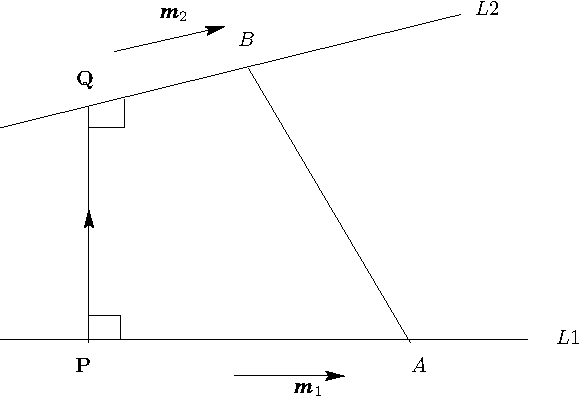
\includegraphics[width=0.5\linewidth]{skewlines.png}
\end{figure}
\noindent
Since $P$ lies on $L_1$ and $Q$ lies on $L_2$, the points should satisfy 
	equations (\ref{eq1}) and (\ref{eq2}), respectively.

\noindent
%$\therefore$
\begin{equation}
\begin{pmatrix}
	p_{1} \\
	p_{2} \\
	p_{3}
\end{pmatrix}
	=
\begin{pmatrix}
	a_{11} + \lambda b_{11} \\
	a_{12} + \lambda b_{12} \\
	a_{13} + \lambda b_{13}
\end{pmatrix}
\end{equation}
	and
\begin{equation}
\begin{pmatrix}
	q_{1} \\
	q_{2} \\
	q_{3}
\end{pmatrix}
	=
\begin{pmatrix}
	a_{21} + \mu b_{21} \\
	a_{22} + \mu b_{22} \\
	a_{23} + \mu b_{23}
\end{pmatrix}
\end{equation}
\begin{align}
	\mathbf{PQ} &= \mathbf{Q} - \mathbf{P} 	\nonumber \\
		&=
\begin{pmatrix}
	a_{21} - a_{11} + \mu b_{21} - \lambda b_{11} \\
	a_{22} - a_{12} + \mu b_{22} - \lambda b_{12} \\
	a_{23} - a_{13} + \mu b_{23} - \lambda b_{13}
\end{pmatrix}
\end{align}
The only unknowns are $\lambda$ and $\mu$. \\

\noindent
Since $\mathbf{PQ}$ is perpendicular to $\mathbf{b_1}$ and $\mathbf{b_2}$:
\begin{equation}
	\mathbf{PQ} \cdot \mathbf{b}_1 = 0 \qquad \text{and} \qquad
	\mathbf{PQ} \cdot \mathbf{b}_2 = 0
\end{equation}
these equations can be solved for $\lambda$ and $\mu$.

\end{document}
